\chapter{Taxonomy of IPP for ML models}
\label{ch:taxonomy}

% ------ IPP overview figure
\begin{figure*}[t]

\begin{tikzpicture}
\node[inner sep=0pt] (overview) at (0,0) {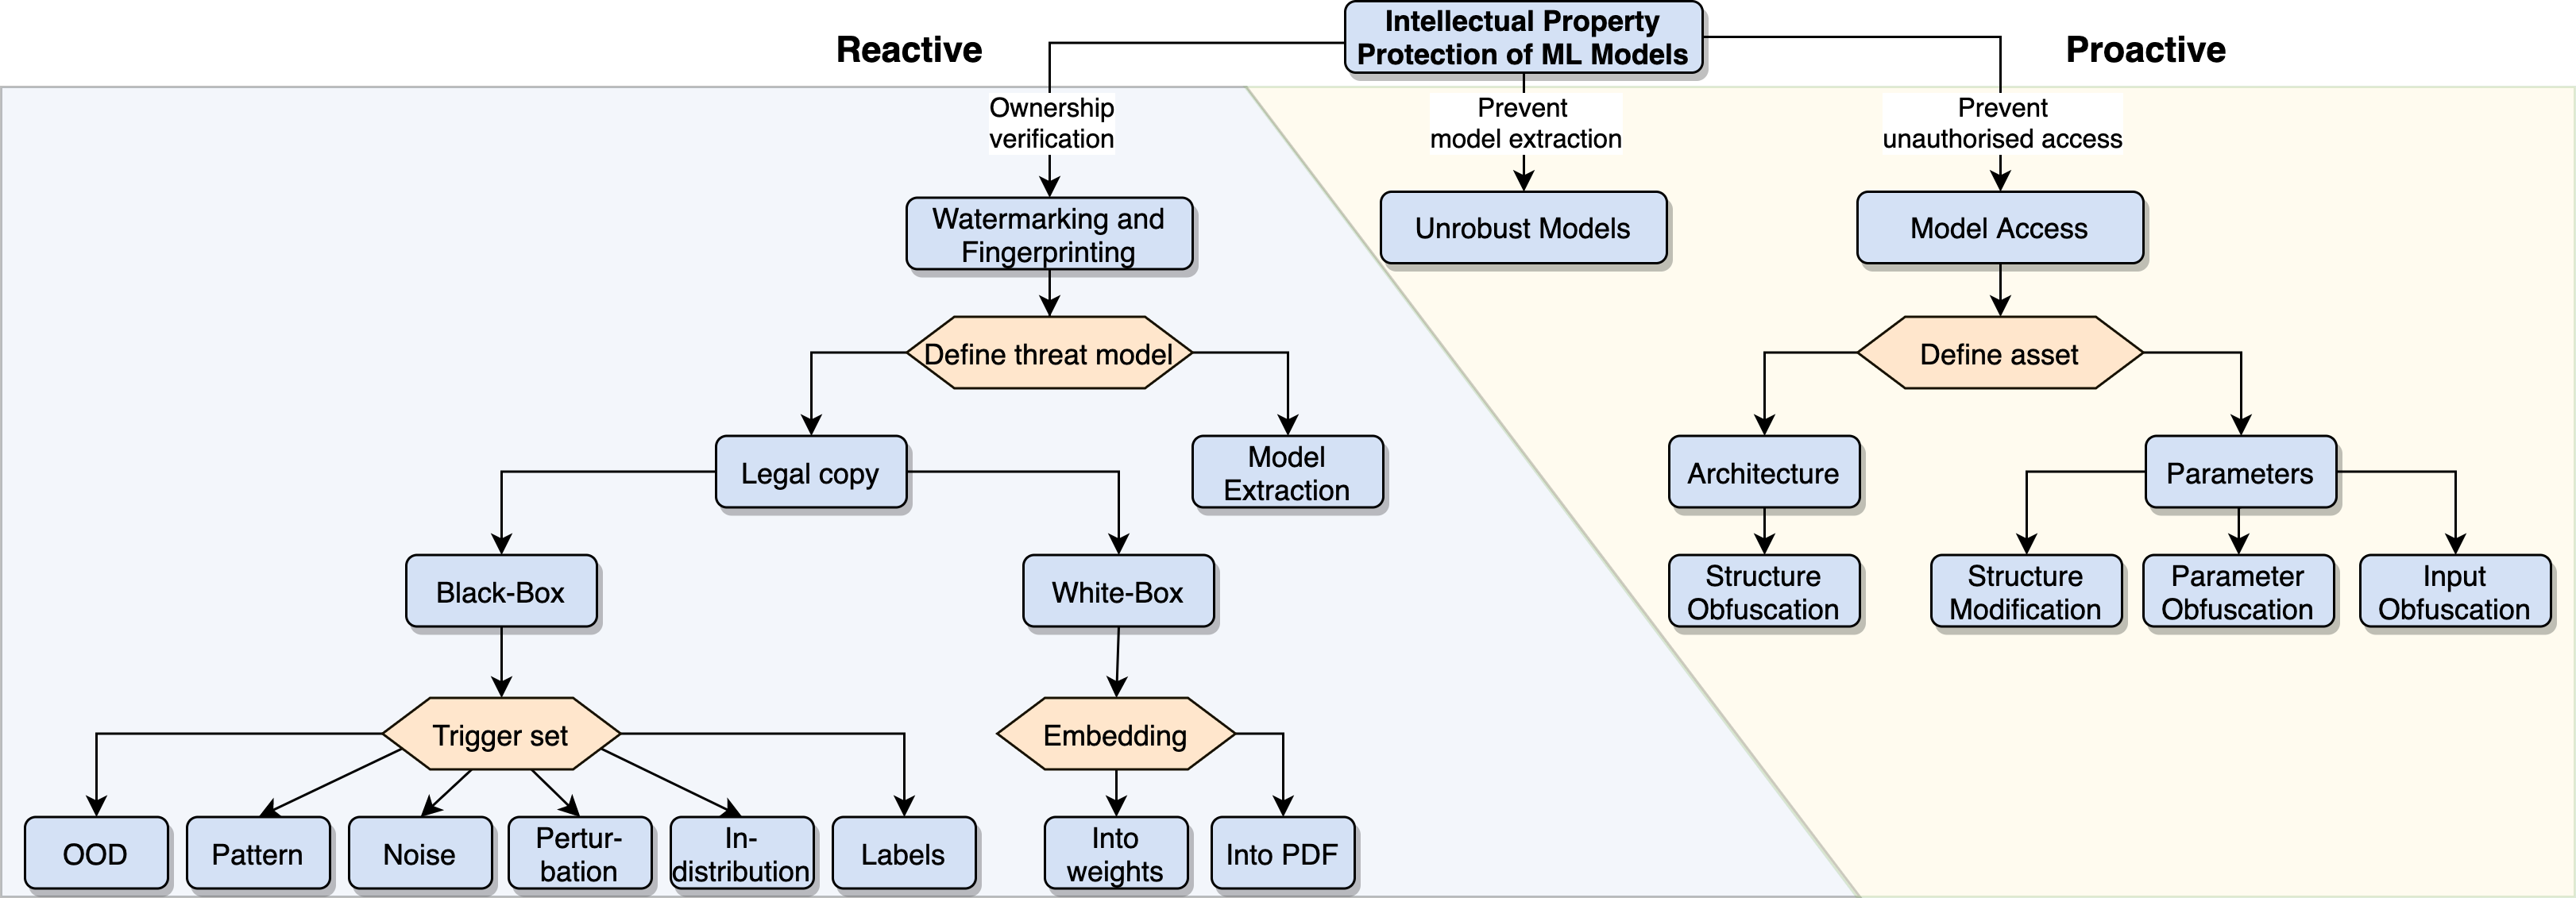
\includegraphics[width=\textwidth]{images/IPP_overview.png}};
%OOD:
\node[inner sep=0pt] (cite1) at (-8.65,-3.25) {\tiny \cite{adi_turning_2018}};
\node[inner sep=0pt] (cite2) at (-8.4,-3.25) {\tiny \cite{zhang_protecting_2018}};
\node[inner sep=0pt] (cite22) at (-8.1,-3.25) {\tiny \cite{yang_effectiveness_2019}};
%pattern:
\node[inner sep=0pt] (cite3) at (-7.7,-3.25) {\tiny \cite{zhang_protecting_2018}};
\node[inner sep=0pt] (cite4) at (-7.4,-3.25) {\tiny \cite{li_piracy_2020}};
\node[inner sep=0pt] (cite5) at (-7.1,-3.25) {\tiny \cite{guo_watermarking_2018}};
\node[inner sep=0pt] (cite6) at (-6.8,-3.25) {\tiny \cite{guo_evolutionary_2019}};
%noise:
\node[inner sep=0pt] (cite7) at (-6.25,-3.25) {\tiny \cite{zhang_protecting_2018}};
\node[inner sep=0pt] (cite8) at (-5.95,-3.25) {\tiny \cite{zhu_secure_2020}};
%perturbation:
\node[inner sep=0pt] (cite9) at (-5.3,-3.25) {\tiny \cite{merrer_adversarial_2019}};
\node[inner sep=0pt] (cite10) at (-5.0,-3.25) {\tiny \cite{li_how_2019}};
\node[inner sep=0pt] (cite11) at (-4.7,-3.25) {\tiny \cite{chen_blackmarks_2019}};
\node[inner sep=0pt] (cite12) at (-5.1,-3.45) {\tiny FP: \cite{zhao_afa_2019}};
\node[inner sep=0pt] (cite13) at (-4.7,-3.45) {\tiny \cite{lukas_deep_2020}};
%in-distr.:
\node[inner sep=0pt] (cite14) at (-3.85,-3.25) {\tiny \cite{namba_robust_2019}};
%trigger labels:
\node[inner sep=0pt] (cite15) at (-3,-3.25) {\tiny \cite{zhong_protecting_2020}};
\node[inner sep=0pt] (cite16) at (-2.7,-3.25) {\tiny \cite{zhang_deeptrigger_2020}};
\node[inner sep=0pt] (cite16) at (-2.4,-3.25) {\tiny \cite{xu_identity_2020}};

%into weights:
\node[inner sep=0pt] (cite17) at (-1.65,-3.25) {\tiny \cite{uchida_embedding_2017}};
\node[inner sep=0pt] (cite18) at (-1.35,-3.25) {\tiny \cite{wang_robust_2020}};
\node[inner sep=0pt] (cite19) at (-1.05,-3.25) {\tiny \cite{wang_watermarking_2020}};
\node[inner sep=0pt] (cite20) at (-0.75,-3.25) {\tiny \cite{feng_watermarking_2020}};
%into pdf:
\node[inner sep=0pt] (cite21) at (-0.3,-3.25) {\tiny \cite{rouhani_deepsigns_2019}};
\node[inner sep=0pt] (cite22) at (0.2,-3.25) {\tiny FP: \cite{chen_deepmarks_2019}};
%Model Extraction:
\node[inner sep=0pt] (cite23) at (1,-1.4) {\tiny \cite{jia_entangled_2020}}; 
\node[inner sep=0pt] (cite24) at (1.3,-1.4) {\tiny \cite{szyller_dawn_2020}};
% man könnte noch diese hinzufügen, aber lasse ich für die version erstmal...
%\node[inner sep=0pt] (cite241) at (1.6,-1.4) {\tiny \cite{wu_watermarking_2020}};
%\node[inner sep=0pt] (cite242) at (1.9,-1.4) {\tiny \cite{zhang_model_2020}};

% Unrobust models
 \node[inner sep=0pt] (cite25) at (1.7,1.15) {\tiny \cite{szentannai_preventing_2019}};
 
%Structure Obfuscation:
\node[inner sep=0pt] (cite101) at (3.35,-1.4) {\tiny \cite{xu_deepobfuscation_2018}};
 
% Structure Modification:
\node[inner sep=0pt] (cite102) at (5.2,-1.4) {\tiny \cite{fan_rethinking_2019}};

% Parameter Encryption & Obfuscation:
\node[inner sep=0pt] (cite103) at (6.13,-1.4) {\tiny \cite{gomez_security_2019}};
\node[inner sep=0pt] (cite104) at (6.43,-1.4) {\tiny \cite{chakraborty_hardware-assisted_2020}};
\node[inner sep=0pt] (cite105) at (6.73,-1.4) {\tiny \cite{alam_deep-lock_2020}};
\node[inner sep=0pt] (cite106) at (7.03,-1.4) {\tiny \cite{tang_deep_2020}};
\node[inner sep=0pt] (cite107) at (7.33,-1.4) {\tiny \cite{lin_chaotic_2020}};

%Input Obfuscation:
\node[inner sep=0pt] (cite108) at (8.1,-1.4) {\tiny \cite{aprilpyone_training_2020}};
\node[inner sep=0pt] (cite109) at (8.4,-1.4) {\tiny \cite{chen_protect_2018}};

\end{tikzpicture}

%    \caption{Taxonomy of IPP protection mechanisms for ML models.}
    \caption{Taxonomy of Intellectual Property Protection mechanisms for Machine Learning models. Note: not all considered papers are referenced in this diagram.}
        \label{fig:overview}
\end{figure*}
% ------ end

In this section, we provide a comprehensive taxonomy of IPP methods for ML models, the threat model and attacks.

We first define our threat model, to then discuss potential schemes to mitigate risks of those threats.
We then provide an overview of attacks against those IPP mechanisms.

\section{Threat Model}
\label{sec:threatmodel}

To define a threat model we first need to understand the motives of an attacker (or adversary or malicious user).
The model owner, i.e. the person that invested resources to obtain an ML model for a specific task, wants to offer the model to some target audience for use.
The most prominent reasons for an attacker to redistribute such a model would be (i) having no (or not enough) training data, expertise, time or computational power to train such a model themself, and/or (ii) the unwillingness to agree with the license terms of the obtained model or the fees for using it in a Machine Learning as a Service (MLaaS) setting.
We call the model that has to be protected the \textit{target model}, and the attacker's model, which arises from the target model, the \textit{adversary model}. As a threat model, we consider either one of the following situations:
% 
\begin{enumerate}
    \item \textbf{Legal copy:} The model owner distributes the model publicly, either for free, e.g. via a platform such as Model Zoo \cite{noauthor_model_nodate}, but with a restrictive license, or for a fee. The attacker then obtains this model and redistributes it via a lucrative API service.
    \item \textbf{Illegal copy:} The model owner distributes the model as a pay-per-query API service. The attacker then performs a Model Extraction Attack and provides his own lucrative API service.
\end{enumerate}

Regardless of how the attacker obtained the model, in both cases, the IP of the model owner is illegally utilised. For both cases, we will discuss methods to protect the IP of the model owner. It is important to differentiate between those two cases, as this has a large impact on selecting potential defence mechanisms. 

\section{IPP Methods}
We developed a comprehensive taxonomy of IPP methods for ML models, depicted in \cref{fig:overview}.

A principal categorisation of model watermarking methods is by \textit{white-box} or \textit{black-box} watermarking methods. White-box approaches embed the watermark in the model parameters or other model characteristics. With that in mind, the model owner would need the get the stolen copy from the attacker for the watermark verification process. This scenario seems unrealistic in most settings (e.g. an attacker offering an API service based on the model never discloses the model itself), and is the likely reason why black-box watermarking tends to be more popular, as the model owner can verify ownership with as little as a set of trigger inputs and the corresponding responses of the adversary model.

A further distinction is between (i) \textit{reactive methods}, which try to react to a threat event, or (ii) \textit{proactive methods}, which means the defender takes initiative, to prevent a threat event.
%Reactive methods include watermarking and fingerprinting, while proactive methods include model access control.
Regarding the goal of the protection, we distinguish methods that enable to verify the ownership of a model, by \textit{model watermarking} and \textit{model fingerprinting}, and are thus \textit{reactive}, and methods that, e.g., want to prevent unauthorised model access, and are thus \textit{proactive}. %TODO: Mimosanet
Ownership verification is a weak form of protection, as it requires the unauthorised usage of the model to be known (or at least suspected), and further requires some form of access to the model. Model access control, on the other hand, shall prevent such illegal use, by rendering the model useless to unauthorised users. This is comparable to preventing unauthorised use of, e.g., software.

Watermarking against the threat of a model extraction attack is mostly achieved by special black-box watermarking techniques that survive such an attack, i.e. the hidden information is "stolen" along with the model itself. In case a user initially obtained a legal copy of the ML model but is then using it in a way not according to the licensing terms, more techniques are available. White-box approaches for this case embed the ownership information directly into the model parameters, or in their probability density function (PDF). Black-box approaches mostly rely on specific input samples, so-called \textit{trigger sets}, that will cause the model to behave in a way that is unexpected for the task, and unknown to the attacker. The techniques mainly differ in the way these triggers are constructed.

Model access control methods can be distinguished by the asset they want to protect. Most work focuses on the protection of the model parameters, either by encryption, other obfuscation techniques, or requiring a specific method to transform the inputs. If the model structure (or architecture) is to be protected, obfuscation techniques for those are employed.

\section{Attack Model} \label{sec:attack-model}
%TODO: make more generic, for all IPP

In \cref{sec:attacks} we will introduce specific attacks against IPP mechanisms, namely \textit{detection}, \textit{overwriting}, \textit{invalidation} and \textit{removal}. Therefore, this section provides the attack models to which we will refer later on. Let us assume that the attacker obtains a legal copy of the target model, and either knows or assumes that the model has an IPP in place.

We consider the following cases as attack models for watermarking:

\begin{itemize}
    \item  
\textbf{Watermark detection:} The attacker wants to detect if there is a watermark in the model, e.g. to then perform a targeted watermark removal or overwriting. If the watermark is not secured with an additional mechanism (e.g. a private key for extraction), the attacker could also claim ownership.
\item \textbf{Watermark overwriting:} The attacker wants to overwrite an existing watermark by placing their own watermark and making the model owner's watermark useless.
\item \textbf{Watermark invalidation:} The attacker wants to disable the watermark function, without actually removing it from the model, so that it cannot be verified. 
%\footnote{An example is an ensemble attack where API services do not respond relying on a single model's prediction, but on several different models so that when triggering, the expected trigger label is not revealed \cite{hitaj_evasion_2019}.}
\item \textbf{Watermark removal:} The attacker wants to modify the model in a way such that the model owner's watermark extraction algorithm will no longer result in proving correct ownership, ownership of the real model owner.
\end{itemize}

Most of these attacks are also valid against \textit{fingerprinting}.

Against \textbf{model access control} mechanisms, an attacker mostly would want to \textbf{remove} or \textbf{invalidate} (or potentially overwrite) the mechanism to gain unauthorised access to use the model (as black-box) or to reveal either the model architecture or model parameters for other purposes.

